\documentclass[12pt]{beamer}

\usetheme{Malmoe}
\usepackage[utf8]{inputenc}
\usepackage{graphicx}
\usepackage{xcolor}
\usepackage{wrapfig} % texlive-latex-extra package
\usepackage{underscore}
\usepackage{listings}

\definecolor{Cyan}{RGB}{0,141,184}
\definecolor{codeblock}{RGB}{220,220,220}

\setbeamercolor{structure}{fg=Cyan}

\setbeamerfont{title}{series=\bfseries,parent=structure}
\setbeamerfont{subtitle}{size=\normalsize,series=\bfseries,parent=structure}
\setbeamerfont{author}{size=\scriptsize,series=\bfseries,parent=structure}
\setbeamerfont{institute}{size=\scriptsize,series=\bfseries,parent=structure}
\setbeamerfont{date}{size=\scriptsize,series=\bfseries,parent=structure}

%\ shell code block style (https://en.wikibooks.org/wiki/LaTeX/Source_Code_Listings)
\lstset{language=sh,
	basicstyle=\ttfamily\scriptsize,
	backgroundcolor=\color{codeblock},
	commentstyle=\color{blue},
	breaklines=true,
	breakatwhitespace=true,
	showstringspaces=false
}

\title{GIS.lab}
\subtitle{news from development of technology for rapid deployment of complete geospatial infrastructure with supercow capabilities}
\author{Ivan Minčík (imincik)}
%\setbeamercovered{transparent} 
%\setbeamertemplate{navigation symbols}{} 
%\logo{} 
\institute{FOSS4G Europe 2015, Como, Italy}
\date{} 
%\subject{}


% document BEGIN
\begin{document}


\begin{frame}
	\titlepage
\end{frame}

\begin{frame}{The Super Cow}
	\textbf{3 years} old, \textbf{100 litres} of milk for \textbf{20 kg of GRASS} daily
	\begin{center}
		
\includegraphics[keepaspectratio=true,height=0.6\textheight]{images/cow.png}
	\end{center}
\end{frame}


\section{Introduction}
\begin{frame}
	\begin{center}
		\LARGE\textbf{Introduction}	
	\end{center}
\end{frame}

\begin{frame}{The Problem}
	\begin{center}
		We always need \textbf{more than only one app} for our GIS work flow
	\end{center}
\end{frame}

\begin{frame}{The Problem}
	\begin{center}
		Deployment and maintenance of \textbf{complex system is hard} even if things are going flawlessly
		\end{center}
\end{frame}

\begin{frame}{The Problem}
	\begin{center}
		which usually they are \textbf{not} (:
	\end{center}
\end{frame}

\begin{frame}{GIS.lab}
	\textbf{Instantly} in production, \textbf{no feeding}
	\begin{center}
		%\ image: cow with QGIS, GRASS and PostGIS in bottles
		
\includegraphics[keepaspectratio=true,height=0.6\textheight]{images/cow.png}
	\end{center}
\end{frame}


\section{What is GIS.lab ?}
\begin{frame}
	\begin{center}
		\LARGE\textbf{What is GIS.lab ?}
	\end{center}
\end{frame}

\begin{frame}{What is GIS.lab ?}
	\textbf{free} technology which can \textbf{instantly} turn pile of metal scrap in to the \textbf{high-end geospatial cluster}
	\begin{center}
		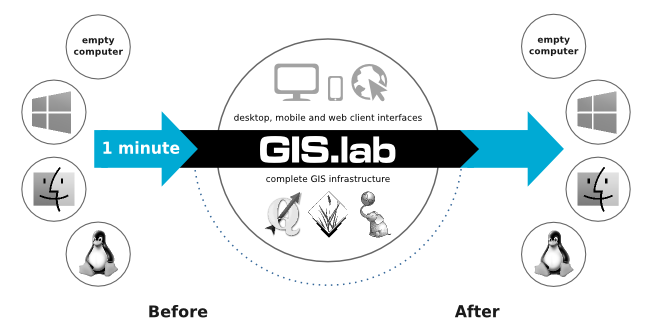
\includegraphics[keepaspectratio=true,height=0.5\textheight]{images/gislab-schema.png}
	\end{center}
\end{frame}

\begin{frame}{What is GIS.lab ?}
	\begin{center}
		and back to \textbf{the same scrap} again
	\end{center}
\end{frame}

\begin{frame}{Features}
	\begin{itemize}[<+->]
		\item \textbf{plug-and-play} deployment
		\item \textbf{central management}
		\item \textbf{desktop, web and mobile} client interfaces
		\item automatic \textbf{clustering and resources sharing}
		\item \textbf{collaboration} tools
		\item fits in your pocket \textbf{pocket}
		\item or \textbf{LAN, data center} and \textbf{cloud}
		\item \textbf{self containing} technology
	\end{itemize}
\end{frame}

\begin{frame}{GIS.lab Cluster Architecture}
	\begin{center}
		%\ image: gis.lab architecture
		
\includegraphics[keepaspectratio=true,height=0.5\textheight]{images/image.png}
	\end{center}
\end{frame}

\begin{frame}{GIS.lab Server}
	%\ server image
	\begin{center}
		
\includegraphics[keepaspectratio=true,height=0.3\textheight]{images/image.png}
	\end{center}
	\begin{itemize}
		\item \textbf{cluster} orchestration
		\item \textbf{data storage} and \textbf{sharing}
		\item \textbf{central} management
		\item \textbf{load balancing} management
		\item \textbf{client launch} support
	\end{itemize}
\end{frame}

\begin{frame}{GIS.lab Clients}
	%\ clients image
	\begin{center}
		
\includegraphics[keepaspectratio=true,height=0.3\textheight]{images/image.png}
	\end{center}
	\begin{itemize}
		\item launching \textbf{from server}
		\item \textbf{user interfaces} for data processing, analysis and collaboration
		\item \textbf{computing power} for cluster
	\end{itemize}
\end{frame}

\begin{frame}{Desktop, Web and Mobile Interfaces}
	\begin{center}
		%\image: desktop + web + mobile schemas
		
\includegraphics[keepaspectratio=true,height=0.5\textheight]{images/image.png}
	\end{center}
\end{frame}


\section{What is new ?}
\begin{frame}
	\begin{center}
		\LARGE\textbf{So, what's new ?}	
	\end{center}
\end{frame}

\begin{frame}
	\begin{center}
		mostly \textbf{everything}
	\end{center}
\end{frame}


\section{Deployment}
\begin{frame}
	\begin{center}
		\LARGE\textbf{Deployment}	
	\end{center}
\end{frame}

\begin{frame}{Automatic deployment}
	\begin{center}
		
\includegraphics[keepaspectratio=true,height=0.4\textheight]{images/ansible.png}
	\end{center}
	\begin{itemize}
		\item \textbf{no requirements on target machine} except SSH
		\item idempotent \textbf{modules, templates}
		\item \textbf{cloud providers} AWS, GCE, Digital Ocean, Azure ...
	\end{itemize}
\end{frame}

\begin{frame}[fragile]{Automatic deployment}
	\begin{center}
		
\includegraphics[keepaspectratio=true,height=0.4\textheight]{images/ansible.png}
	\end{center}

   \lstset{language=sh}
	\begin{lstlisting}
		$ ansible-playbook
		  --inventory=gislab.inventory
		  --private-key=~/.ssh/id_rsa
		  system/gislab.yml
	\end{lstlisting}
\end{frame}

\begin{frame}[fragile]{Virtual Machine - Development and Testing}
	\begin{center}
		
\includegraphics[keepaspectratio=true,height=0.4\textheight]{images/vagrant.png}
		
\includegraphics[keepaspectratio=true,height=0.4\textheight]{images/virtualbox.png}
		
\includegraphics[keepaspectratio=true,height=0.4\textheight]{images/ansible.png}
	\end{center}

   \lstset{language=sh}
	\begin{lstlisting}
		$ vagrant up
		Bringing machine 'gislab_vagrant' up with 'virtualbox' provider...
		==> gislab_vagrant: Importing base box 'precise-canonical'...
		==> gislab_vagrant: Running provisioner: install (ansible)...
	\end{lstlisting}
\end{frame}

\begin{frame}{GIS.lab Unit - End User Deployment}
	\begin{center}
		
\includegraphics[keepaspectratio=true,height=0.5\textheight]{images/gislab-unit.png}
	\end{center}
	\begin{itemize}
		\item portable, pocket size
		\item plug-and-play
		\item automatic adaptation to host network
	\end{itemize}
\end{frame}


\section{Client Interfaces}
\begin{frame}
	\begin{center}
		\LARGE\textbf{Client Interfaces}
	\end{center}
\end{frame}

\begin{frame}{Client Interfaces}
	\begin{center}
		%\ image: client interfaces
		
\includegraphics[keepaspectratio=true,height=0.5\textheight]{images/image.png}
	\end{center}
\end{frame}


\begin{frame}
	\begin{center}
		\LARGE\textbf{Desktop}	
	\end{center}
\end{frame}

\begin{frame}{Machines Launch}
	\begin{center}
		%\ image: boot from server
		
\includegraphics[keepaspectratio=true,height=0.5\textheight]{images/image.png}
	\end{center}
	\begin{itemize}
		\item \textbf{network boot} (PXE, HTTP)
		\item \textbf{clean system} after each launch
		\item \textbf{no HDD} required
	\end{itemize}
\end{frame}

\begin{frame}{Physical or Virtual Mode}
	\begin{center}
		%\ image: Physycal or Virtual Mode
		
\includegraphics[keepaspectratio=true,height=0.5\textheight]{images/image.png}
	\end{center}
	\begin{itemize}
		\item \textbf{physical mode}: best performance, original OS is temporary lost
		\item \textbf{virtual mode}: any OS, original OS and GIS.lab are available
	\end{itemize}
\end{frame}

\begin{frame}{Office Productivity Suite}
	\begin{center}
		%\ image: desktop screenshot with writer, browser, chat ...
		
\includegraphics[keepaspectratio=true,height=0.5\textheight]{images/image.png}
	\end{center}
	\begin{itemize}
		\item \textbf{office} suite
		\item \textbf{Internet} browser, \textbf{chat}, ...
	\end{itemize}
\end{frame}

\begin{frame}{Geospatial Suite}
	\begin{center}
		%\ image: desktop client screenshot with QGIS, GRASS ...
		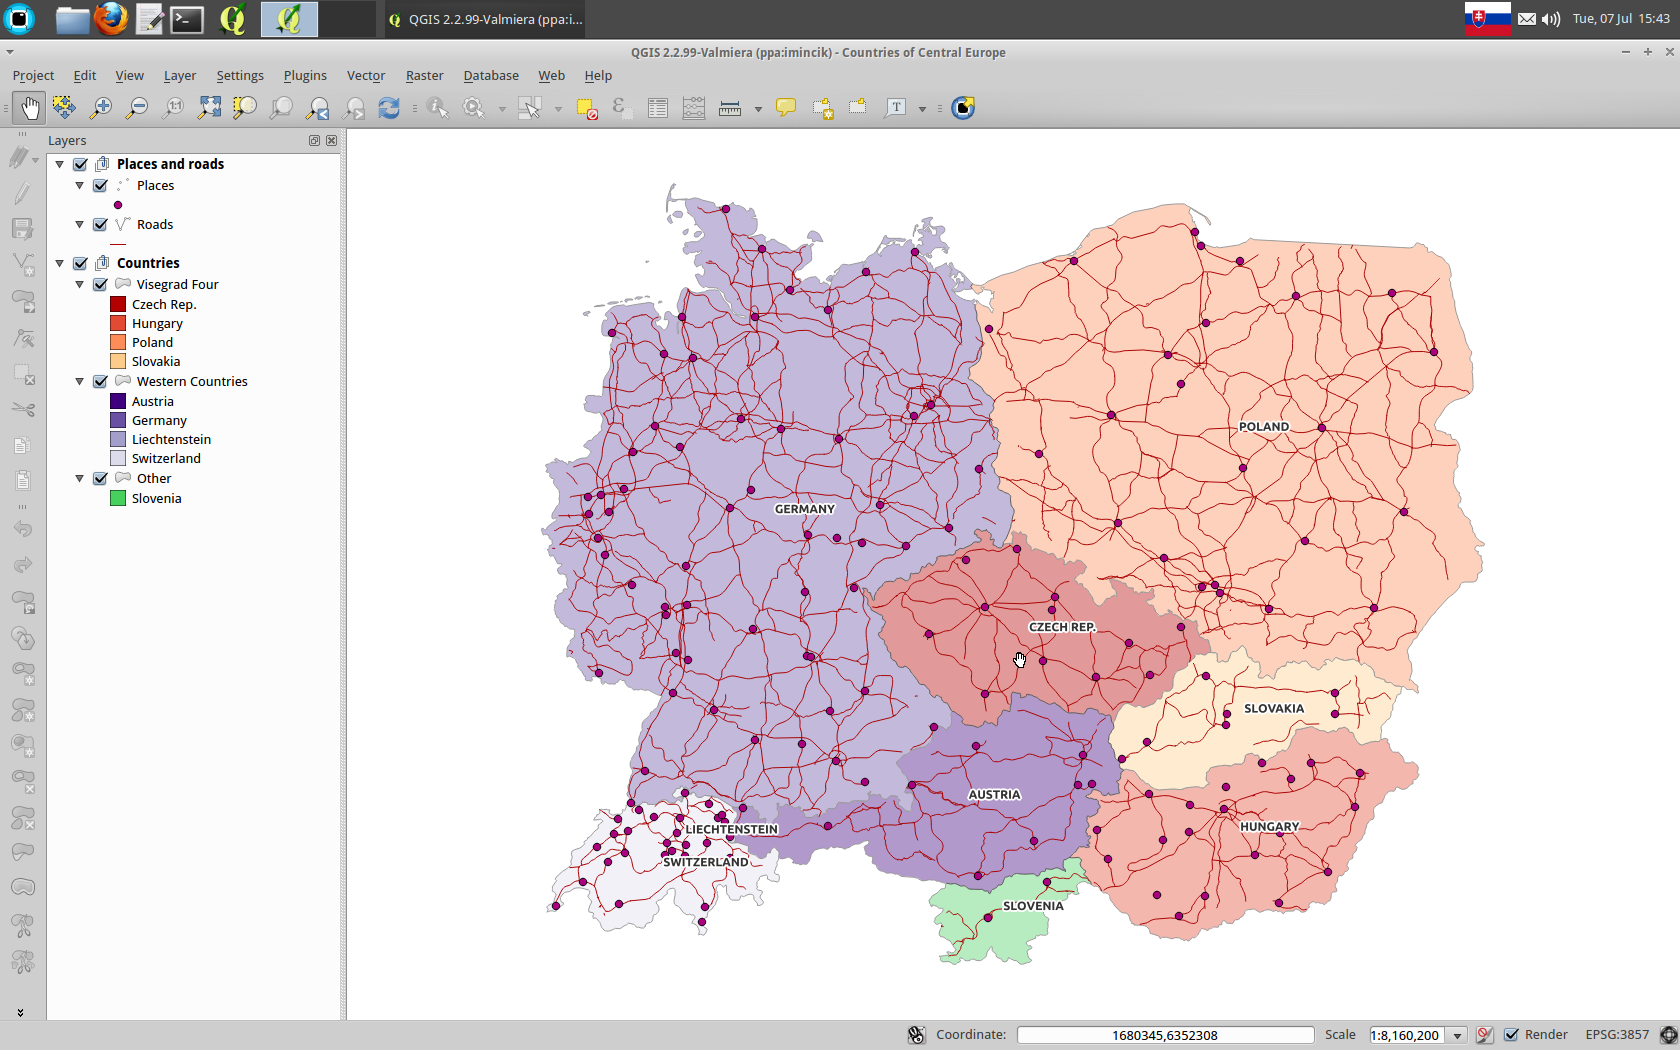
\includegraphics[keepaspectratio=true,height=0.5\textheight]{images/gislab-desktop.png}
	\end{center}
	\begin{itemize}
		\item \textbf{QGIS} as \textbf{The geospatial project IDE}
		\item \textbf{QGIS} for data access and processing
		\item \textbf{GRASS 7} for analysis
		\item \textbf{PostGIS} or \textbf{SpatiaLite} for storage
	\end{itemize}
\end{frame}

\begin{frame}{Maps Publishing}
	\begin{center}
		%\ image: gis.lab web plugin
		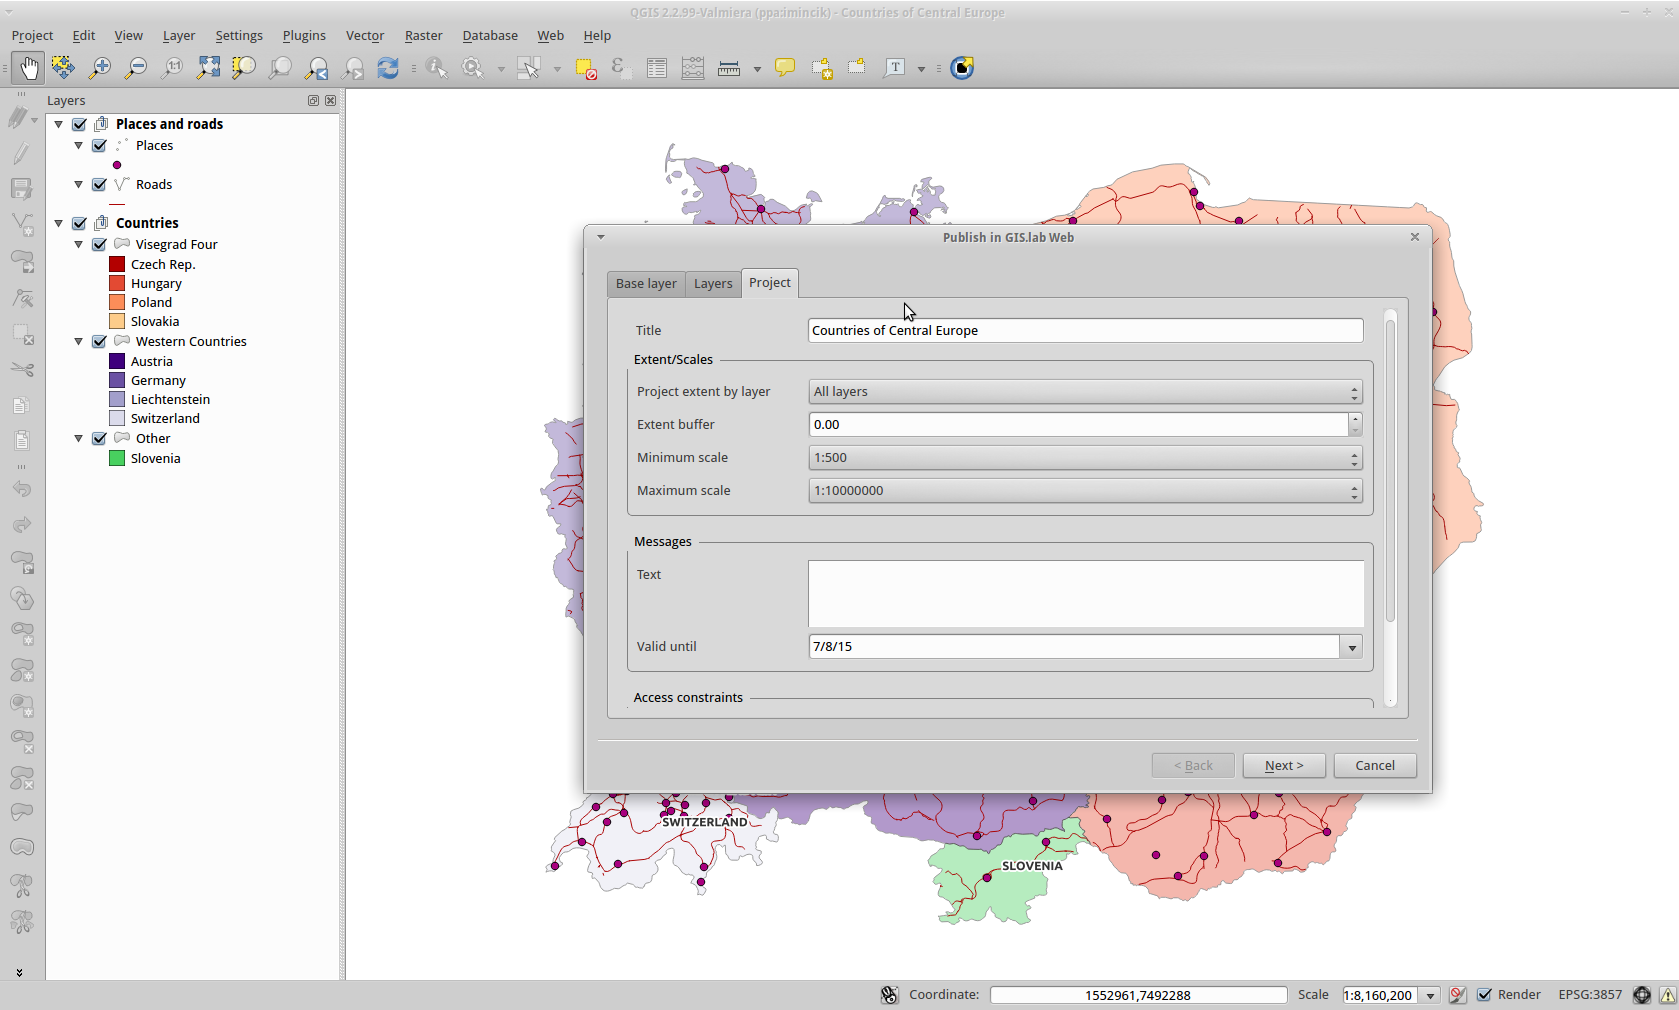
\includegraphics[keepaspectratio=true,height=0.5\textheight]{images/gislab-publish.png}
	\end{center}
	\begin{itemize}
		\item direct publishing to \textbf{web} or \textbf{mobile} from \textbf{QGIS project}
		\item simple \textbf{wizard}
	\end{itemize}
\end{frame}

\begin{frame}[fragile]{Customization}
	\lstset{language=sh}
	\begin{lstlisting}
		$ cp /opt/gislab/client-desktop                  # backup
		     /mnt/backup/client-desktop.backup
		
		$ gislab-client-shell -i   # enter client env
		$ apt-get install gedit    # install Gedit
		$ exit                     # exit client env
		$ gislab-client-image      # deploy updated client image
		
		$ rm -rf /opt/gislab/client-desktop
		  &&
		  mv /mnt/backup/client-desktop.backup
		     /opt/gislab/client-desktop                  # rollback
	\end{lstlisting}

	\begin{itemize}
		\item \textbf{isolated environment}, using \textbf{standard tools}
		\item \textbf{central} system distribution, \textbf{rollback}
	\end{itemize}
\end{frame}

\begin{frame}[fragile]{Booster File System}
	\textbf{Test writing of 2 GB file}
	\\
	HDD
	\lstset{language=sh}
	\begin{lstlisting}
		$ dd if=/dev/zero of=/tmp/test.f bs=1M count=2048
		  2147483648 bytes (2,1 GB) copied, 24,8055 s, 86,6 MB/s
	\end{lstlisting}

	Booster
	\lstset{language=sh}
	\begin{lstlisting}
		$ dd if=/dev/zero of=~/Booster/test.f bs=1M count=2048
		  2147483648 bytes (2,1 GB) copied, 0,582147 s, 3,7 GB/s
	\end{lstlisting}

	\begin{itemize}
		\item \textbf{super fast} file system in RAM
		\item ideal for \textbf{temporary files}
	\end{itemize}
\end{frame}

\begin{frame}
	\begin{center}
		\LARGE\textbf{Web and Mobile}
	\end{center}
\end{frame}

\begin{frame}{Web and Mobile}
	\begin{center}
		%\ image: web and mobile client screenshots
		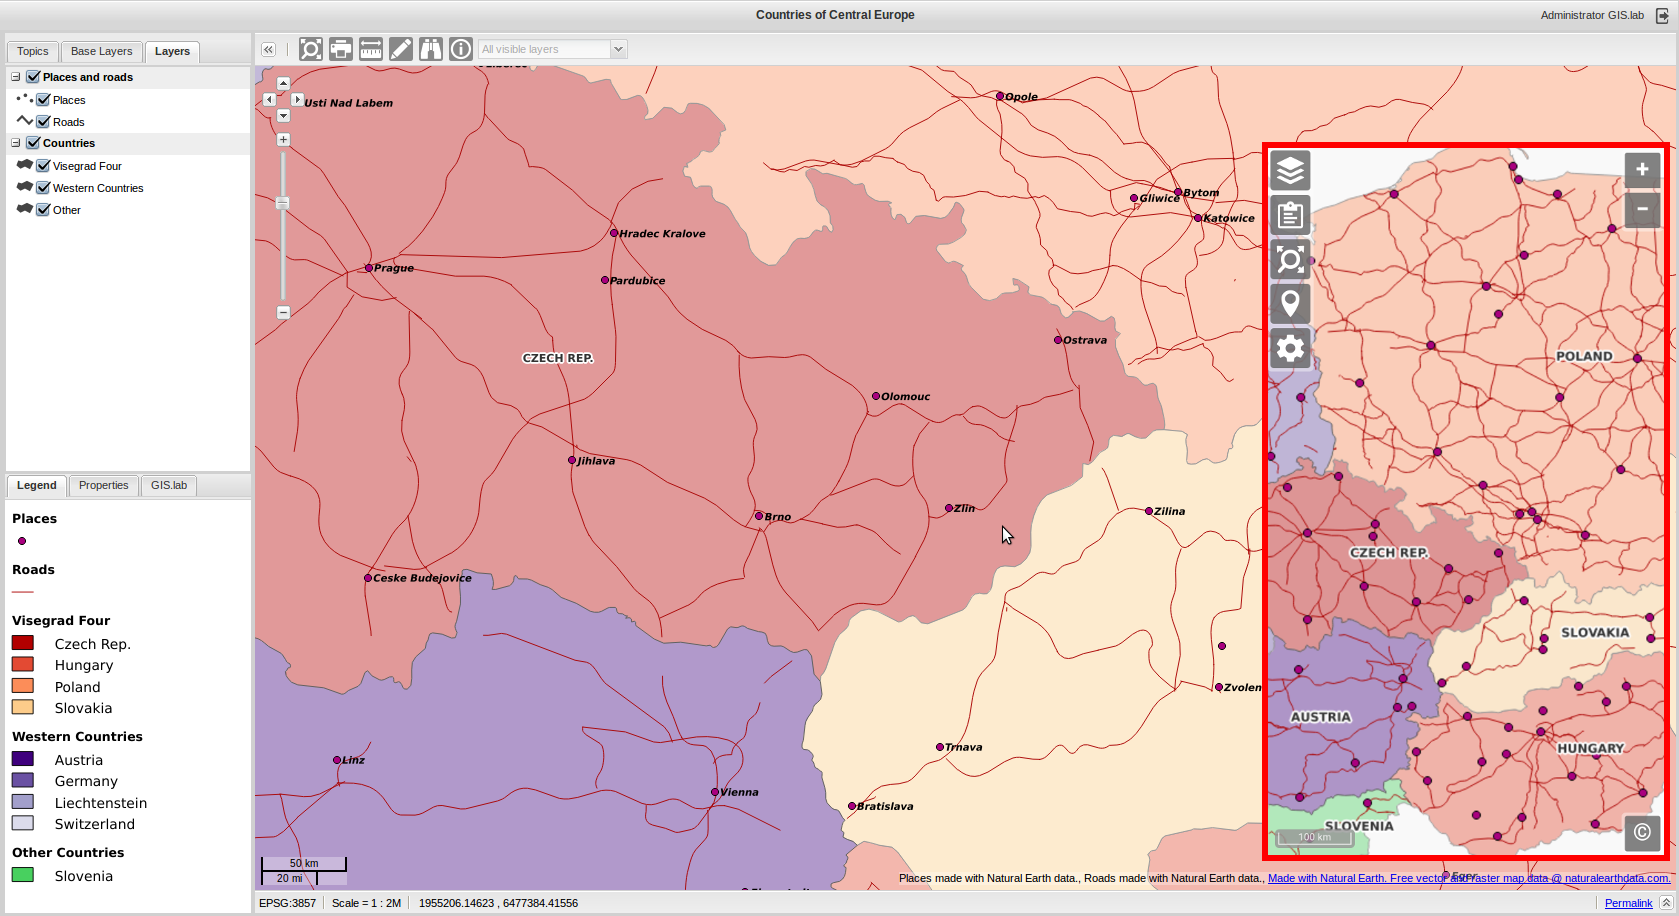
\includegraphics[keepaspectratio=true,height=0.5\textheight]{images/gislab-web+mobile.png}
	\end{center}
	\begin{itemize}
		\item \textbf{themes}, \textbf{base} and \textbf{overlay} layers
		\item advanced \textbf{search} forms
		\item \textbf{print} outputs
		\item vector features \textbf{drawing} and \textbf{sharing}
	\end{itemize}
\end{frame}


\section{Cluster}
\begin{frame}
	\begin{center}
		\LARGE\textbf{Cluster}	
	\end{center}
\end{frame}

\begin{frame}{Automatic Cluster Orchestration}
	\begin{center}
		
\includegraphics[keepaspectratio=true,height=0.5\textheight]{images/serf.png}
	\end{center}
	\begin{itemize}
		\item formed by \textbf{server} and \textbf{client machines}
		\item \textbf{decentralized} cluster \textbf{membership} and \textbf{failure detection} system based on GOSSIP protocol
	\end{itemize}
\end{frame}

\begin{frame}[fragile]{Basic Information About Machines}
	\lstset{language=sh}
	\begin{lstlisting}
		$ gislab-cluster members					# format text or json 

		server.gis.lab  192.168.15.5:7946 
		                alive  role=server

		c50             192.168.15.50:7946
		                alive
		                role=client,worker=yes,session-active=user1

		c51             192.168.15.51:7946
		                left
		                role=client,worker=yes
	\end{lstlisting}
\end{frame}

\begin{frame}[fragile]{Events and Queries}
	\textbf{Syntax}
	\lstset{language=sh}
	\begin{lstlisting}
		$ gislab-cluster event <EVENT-NAME>
		$ gislab-cluster query <QUERY-NAME>		
	\end{lstlisting}

	\textbf{Reboot event}
	\lstset{language=sh}
	\begin{lstlisting}
		$ gislab-cluster event reboot
	\end{lstlisting}
\end{frame}

\begin{frame}[fragile]{Parallel Commands Execution}
	\textbf{Example installation of Gedit package on all client machines}
	\lstset{language=sh}
	\begin{lstlisting}
		$ MACHINES="$(
		    gislab-cluster members -tag role=client -status=alive
		    | awk -F " " '{printf "%s ", $1}'
		  )"

		$ parallel-ssh
		  -O StrictHostKeyChecking=no -i -H "$MACHINES"

		  sudo DEBIAN_FRONTEND=noninteractive
		  apt-get install -y --no-install-recommends gedit
		  ...
		  [1] 23:02:57 [SUCCESS] c51
		  [1] 23:02:57 [SUCCESS] c51
		  ...
	\end{lstlisting}
\end{frame}

\begin{frame}{Stronger With Each Client Machine}
	\textbf{Universal usage of each machine - full hardware potential utilization}
	\begin{itemize}
		\item desktop working environment
		\item cluster worker node (OWS services, parallel tasks)
	\end{itemize}
\end{frame}

\begin{frame}[fragile]{Stronger With Each Client Machine}
	\textbf{OWS load balancing}

	\lstset{language=sh}
	\begin{lstlisting}
		$ while true; do
		    curl "http://ms.gis.lab:90/cgi-bin/qgis_mapserv?
		      SERVICE=WMS&REQUEST=GetCapabilities"
		  done
	\end{lstlisting}
	\begin{center}
		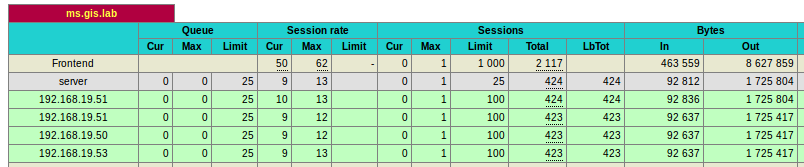
\includegraphics[keepaspectratio=true,width=\textwidth]{images/haproxy-stats.png}
	\end{center}
\end{frame}


\section{Other}
\begin{frame}
	\begin{center}
		\LARGE\textbf{Other}
	\end{center}
\end{frame}

\begin{frame}[fragile]{Integration Test Suite}
	\lstset{language=sh}
	\begin{lstlisting}
		$ vagrant provision --provision-with test
		...
		TASK: [basic-server-configuration-test | Test if ordinary test user account exists in PostgreSQL]
		...
		TASK: [service-dns-test | Test 'gis.lab' DNS records are resolved]
		...
		TASK: [service-mapserver-test | Test WMS GetCapabilies request with example GIS.lab project]
		...
		TASK: [service-mapserver-test | Test WMS GetMap request with example GIS.lab project]
		...
	\end{lstlisting}
\end{frame}

\begin{frame}{Where to Use ?}
	\begin{itemize}
		\item \textbf{schools}: central management, maintenance-free clients
		\item \textbf{small projects}: immediate deployment of complete solution
		\item \textbf{crisis management}: standalone system, working w/o Internet
	\end{itemize}
\end{frame}

\begin{frame}{Future Plans}
	\begin{itemize}
		\item integration of \textbf{WPS} services
		\item better \textbf{GRASS} integration
		\item \textbf{web administration} interface
		\item \textbf{AWS} provider rewrite
		\item \textbf{web client} rewrite with \textbf{OL 3}
		\item update to \textbf{Ubuntu 16.04} and \textbf{systemd}
	\end{itemize}
\end{frame}


\section{Summary}
\begin{frame}
	\begin{center}
		\LARGE\textbf{Summary}
	\end{center}
\end{frame}

\begin{frame}{10 Minutes From Crap to Mobile App for Free}
	\begin{center}
		
\includegraphics[keepaspectratio=true,height=0.5\textheight]{images/image.png}
	\end{center}
\end{frame}

\begin{frame}
	\begin{center}
		\textbf{http://web.gislab.io}
	\end{center}
\end{frame}


% document END
\end{document}